\documentclass[12pt]{tdtp}
\usepackage{tabularx,colortbl}
\usepackage{multirow}
\usepackage{listings}
\lstset{
	language=VHDL,
basicstyle=\tiny\ttfamily}
\definecolor{light-gray}{gray}{0.96}
\definecolor{pageheading-gray}{gray}{0.2}
\definecolor{dark-gray}{gray}{0.45}
\definecolor{dark-green}{rgb}{0.245,0.121,0.0}

\newcommand{\auteur}{Cedric Lemaitre}
\newcommand{\couriel}{c.lemaitre58@gmail.com}
\newcommand{\promo}{Bachelor in Computer Vision}
\newcommand{\annee}{2016-2017}
\newcommand{\matiere}{Image Processing}

\newcommand{\tdtp}{Labs 3}
\renewcommand{\sujet}{Morphogical mathematics}


\begin{document}
\titre

%%%%%%%%%%%%
\Exo
Aim: analyse the effects of the basic operators.
\\
\textbf{Don't use the matlab function, write your own code}
\begin{itemize}
	\item load the image "hubble"
	\item binarize this image
	\item study the effect of with different size of structuring elements with the erosion oprerator
	\item apply the same approach for dilatation, opening and closing
	\item propose a method to measure the granulometry
i\end{itemize}


\begin{figure}[h!]
	\begin{center}
		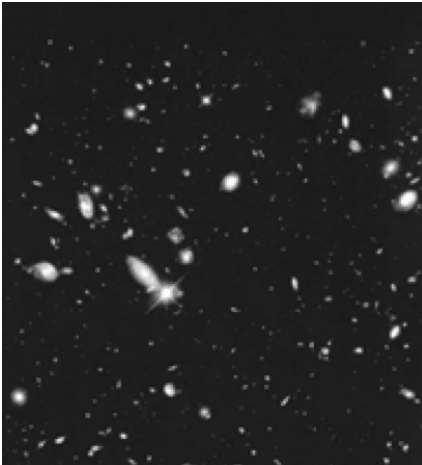
\includegraphics[scale=0.5]{images/hubble.png}
		\caption{Hubble}
		\label{Galaxy}
	\end{center}
\end{figure}


%%%%%%%%%%%%
\newpage 
\Exo

Aim : propose extensions of binary Morphological Mathematics operators\\

\textbf{Don't use the matlab function, write your own code}

\begin{itemize}
	\item propose extensions of binary Morphological Mathematics operators to gray levels images
	\item propose a gradient filter based on MM operators
\end{itemize}

\begin{figure}[h!]
	\begin{center}
		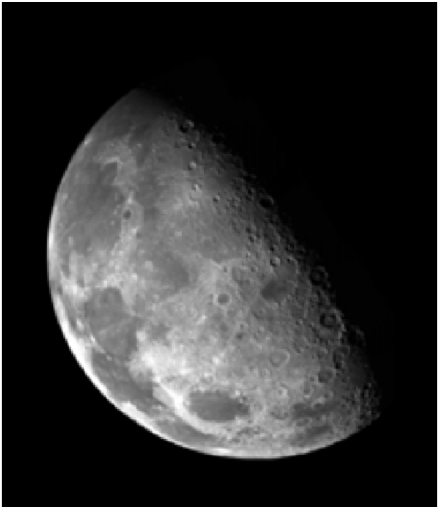
\includegraphics[scale=0.5]{images/moon.png}
		\caption{Moon}
		\label{mri}
	\end{center}
\end{figure}


%%%%%%%%%%%%%%%%%%%%%%%%%%%%%%%%%%
\end{document}
